\documentclass{article}
\usepackage{tikz}
\usetikzlibrary{shapes.geometric}
\usepackage{opensans}

\begin{document}
We are working on
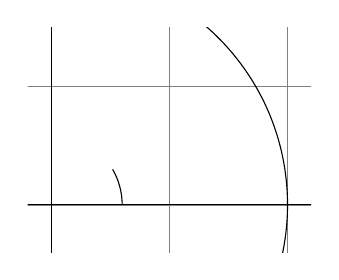
\begin{tikzpicture}[scale = 3]
    \clip (-0.1,-0.2) rectangle (1.1,0.75);
    \draw[step = .5cm, gray, very thin] (-1.4,-1.4) grid (1.4,1.4);
    \draw (-1.5, 0) -- (1.5, 0);
    \draw (0, -1.5) -- (0, 1.5);
    \draw (0, 0) circle [radius = 1cm];
    \draw (3mm,0mm) arc [start angle=0, end angle=30, radius=3mm];
\end{tikzpicture}

\begin{tikzpicture}
    \draw (-1.5, 0) -- (1.5, 0);
    \draw (0, -1.5) -- (0, 1.5);
    \draw (-1, 0) .. controls (-1, 0.555) and (-0.555, 1) .. (0, 1)
                  .. controls (0.555, 1) and (1, 0.555) .. (1, 0);
\end{tikzpicture}

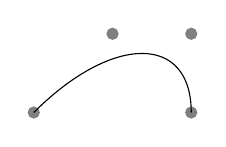
\begin{tikzpicture}
    \filldraw [gray] (0, 0) circle [radius = 2pt]
                     (1, 1) circle [radius = 2pt]
                     (2, 1) circle [radius = 2pt]
                     (2, 0) circle [radius = 2pt];
    \draw (0, 0) .. controls (1, 1) and (2,1) .. (2, 0);
\end{tikzpicture}

Test {\Huge bla

\begin{tikzpicture}[baseline = (O.base), scale = 2ex/1cm, every node/.style={transform shape}]
%\begin{tikzpicture}[scale = 2ex/1cm, every node/.style={transform shape}]
    \filldraw [fill = white, draw = black] (0, 0) circle [radius = 0.5cm];
    \node (O) at (0, 0) {\fontfamily{fos}\fontseries{b}\fontsize{0.5cm}{0.6cm}\selectfont 2};
\end{tikzpicture}
}
bla.

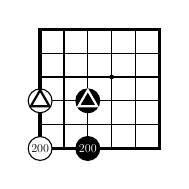
\begin{tikzpicture}[scale = 2ex/1cm, every node/.style={transform shape}]
    \draw (0, 0) grid [step = 1] (5, 5);
    \draw [very thick] (0, 0) rectangle (5, 5);
    \fill (3, 3) circle [radius = 0.1cm];
    \filldraw [fill = white, draw = black] (0, 0) circle [radius = 0.5cm];
    \node at (0, 0) {\fontfamily{fos}\fontseries{b}\fontsize{0.5cm}{0.6cm}\selectfont 200};
    \filldraw [black] (2, 0) circle [radius = 0.5cm];
    \node[white] at (2, 0) {\fontfamily{fos}\fontseries{b}\fontsize{0.5cm}{0.6cm}\selectfont 200};    
    \filldraw [fill = white, draw = black] (0, 2) circle [radius = 0.5cm];
    \node [thick, regular polygon, regular polygon sides=3, minimum size=0.9cm, draw] at (0, 2) {};
    \filldraw [black] (2, 2) circle [radius = 0.5cm];
    \node [thick, white, regular polygon, regular polygon sides=3, minimum size=0.9cm, draw] at (2, 2) {};
\end{tikzpicture}

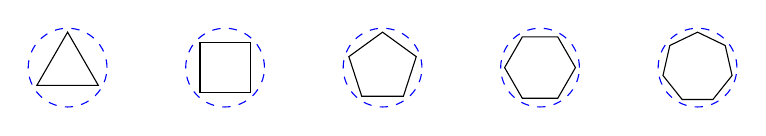
\begin{tikzpicture}
\foreach \a in {3,...,7}{
\draw[blue, dashed] (\a*2,0) circle(0.5cm);
\node[regular polygon, regular polygon sides=\a, minimum size=0.9cm, draw] at (\a*2,0) {};
}
\end{tikzpicture}

\end{document}

